\documentclass{article}
\usepackage{tikz}
\usetikzlibrary{graphs, graphs.standard, quotes, arrows.meta}

\begin{document}

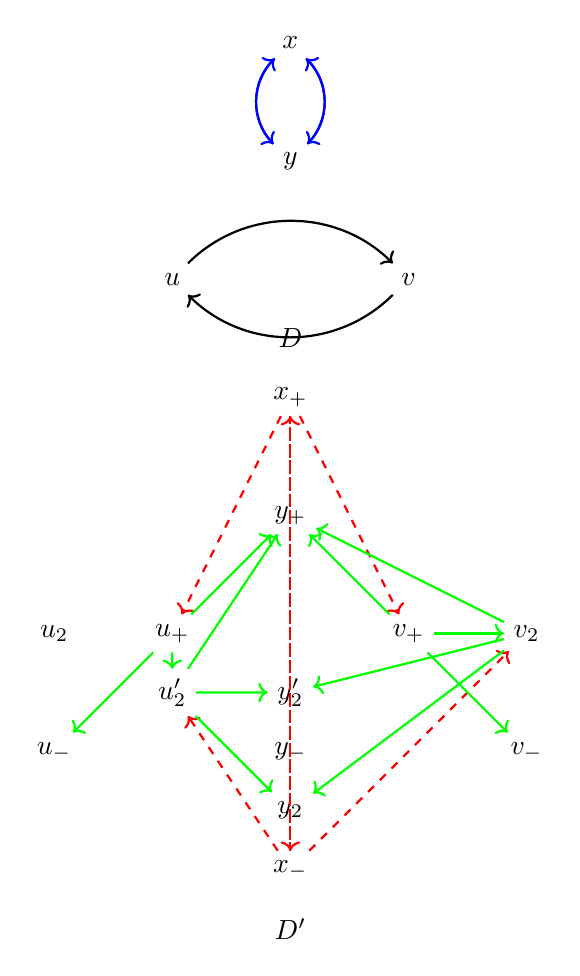
\begin{tikzpicture}[scale=1.5]
    % Define nodes
    \node (x) at (0, 2) {$x$};
    \node (y) at (0, 1) {$y$};
    \node (u) at (-1, 0) {$u$};
    \node (v) at (1, 0) {$v$};

    % Draw edges
    \draw[blue, thick, ->] (x) edge[bend left=45,""] (y);
    \draw[blue, thick, ->] (y) edge[bend left=45,""] (x);
    \draw[blue, thick, ->] (x) edge[bend right=45,""] (y);
    \draw[blue, thick, ->] (y) edge[bend right=45,""] (x);
    \draw[black, thick, ->] (u) edge[bend left=45,""] (v);
    \draw[black, thick, ->] (v) edge[bend left=45,""] (u);

    % Label nodes
    \node at (0, -0.5) {$D$};

    % Second part of the diagram
    \begin{scope}[yshift=-3cm]
        % Define nodes
        \node (x+) at (0, 2) {$x_+$};
        \node (y+) at (0, 1) {$y_+$};
        \node (u+) at (-1, 0) {$u_+$};
        \node (u2+) at (-2, 0) {$u_2$};
        \node (u2-) at (-2, -1) {$u_{-}$};
        \node (y-) at (0, -1) {$y_-$};
        \node (v+) at (1, 0) {$v_+$};
        \node (v2+) at (2, 0) {$v_2$};
        \node (v2-) at (2, -1) {$v_{-}$};
        \node (x-) at (0, -2) {$x_-$};
        \node (y2+) at (0, -0.5) {$y'_2$};
        \node (y2-) at (0, -1.5) {$y_2$};
        \node (u2+) at (-1, -0.5) {$u'_2$};

        % Draw edges
        \draw[red, dashed, thick, ->] (x+) -- (u+);
        \draw[red, dashed, thick, ->] (x+) -- (v+);
        \draw[red, dashed, thick, ->] (x+) -- (x-);
        \draw[red, dashed, thick, ->] (x-) -- (u2+);
        \draw[red, dashed, thick, ->] (x-) -- (v2+);
        \draw[red, dashed, thick, ->] (x-) -- (x+);
        \draw[green, thick, ->] (u+) -- (u2+);
        \draw[green, thick, ->] (u+) -- (u2-);
        \draw[green, thick, ->] (u+) -- (y+);
        \draw[green, thick, ->] (u2+) -- (y2+);
        \draw[green, thick, ->] (u2+) -- (y2-);
        \draw[green, thick, ->] (u2+) -- (y+);
        \draw[green, thick, ->] (v+) -- (y+);
        \draw[green, thick, ->] (v+) -- (v2+);
        \draw[green, thick, ->] (v+) -- (v2-);
        \draw[green, thick, ->] (v2+) -- (y2+);
        \draw[green, thick, ->] (v2+) -- (y2-);
        \draw[green, thick, ->] (v2+) -- (y+);

        % Label nodes
        \node at (0, -2.5) {$D'$};
    \end{scope}
\end{tikzpicture}

\end{document}